\documentclass[a4paper]{scrartcl}

\usepackage{amsmath}
\usepackage{amsfonts}
\usepackage{xcolor}
\usepackage{graphicx}
\usepackage{listings}


\newcommand{\elbo}{\mathcal{L}}
\newcommand{\E}{\mathbb{E}}
\newcommand{\p}{\mathbb{P}}
\newcommand{\q}{q}

\title{Assignment 2AD, 2025}
\subtitle{DD2434 Machine Learning, Advanced Course}
\author{
Bruno Carchia \\
\texttt{carchia@kth.se}
}

\begin{document}
\maketitle

\section*{D Section}
\subsection*{Question D.1}
I chose the dot product similarity as similarity function
\[
Y = W X \quad Y \in R^{d \times n} 
\]
d representes the dimensionality of the data while n is the number of data in the data set and k is the new dimensionality of the data.
\[
S = Y^T Y = (W X)^T (W X) = X^T ( W^T W ) X = X^T X
\]
S matrix is the Gram matrix.\\
Why this choice is meaningful:
\begin{itemize}
    \item Interpretation \(\rightarrow\)the dot product measures the alignment between two MEPs' voting patterns. Higher values indicate greater agreement.
    \item Domain appropriateness \(\rightarrow\) in voting behavior analysis, we care about agreement on specific votes. The dot product naturally captures co-voting patterns ( when both MEPs vote the same way, it contributes positively to similarity )
    \item Simplicity \(\rightarrow\) unlike cosine similarity, the dot product doesn't normalize by magnitude, which can be meaningful here ( MEPs who vote more often and agree more should have higher similarity )
\end{itemize}
Transformation steps required for our similarity computation:
\begin{itemize}
    \item Encoding of the EPG column 
    \begin{itemize}
        \item 0 (not an MEP) → exclude from computation
        \item 1 (for) →  +1
        \item 2 (against) → -1
        \item 3 (abstention) → 0
        \item 4 (absent) → 0
        \item 5 (did not vote) → 0
        \item 6 (motivated) → 0 
    \end{itemize}
"For" and "Against" are opposite positions (+1, -1) 
    \item Filtering → MEPs with a very low participation rate are ignored
    \item Missing Data → for each pair of MEPs, only include votes where BOTH MEPs were present and voted. This ensures we're measuring similarity based on actual voting decisions, not absence patterns.
    \item Center → subtract each MEP's mean vote in order to remove the baseline voting tendency of each MEP.
    \item Normalize → divide by L2 norm in order to make similarity values comparable across MEP pairs with different participation rates.
\end{itemize}
I selected MEPs from both the EP8 (2014-2019) and EP9 (2019-2022) sessions, applying a minimum participation threshold of 30\% This resulted in a subset of 1,520 MEPs who voted on 10,251 recorded votes, yielding approximately 2.3 million pairwise similarity comparisons.
Reasons:
\begin{itemize}
    \item combining two consecutive parliamentary sessions provides a broader temporal perspective, allowing the analysis to capture both stable political alignments and potential shifts in voting behavior across time.
    \item the 30\% participation threshold ensures that similarity estimates are based on a substantial number of co-voted issue
    \item the computed similarity matrix shows expected properties: perfect self-similarity (diagonal \(\approx\) 1.0), symmetry, and a reasonable distribution of similarities (mean = 0.14, std = 0.27) with both high agreement (max = 0.998) and strong opposition (min = -0.42) represented.
\end{itemize}
\subsection*{Question D.2}
We want to find the latent matrix \(X \in R^{k \times n}\) such that \(S = X^T X\).\\
The similarity matrix \(S\) is symmettic positive semi-definite , so its eigen-decomposition is
\[
S = U \Lambda U^{-1} = U \Lambda U^{T} = (\Lambda^{0.5} U^T)^T (\Lambda^{0.5} U^T)
\]
The non negative eigenvalues of S are sorted in descending oder in the diagonal of \(\Lambda\), we can take the \(k \times n\) matrix X to be 
\[
X = I_{k \times n} \Lambda^{0.5} U^T
\]
\begin{figure}[h!]
    \centering
    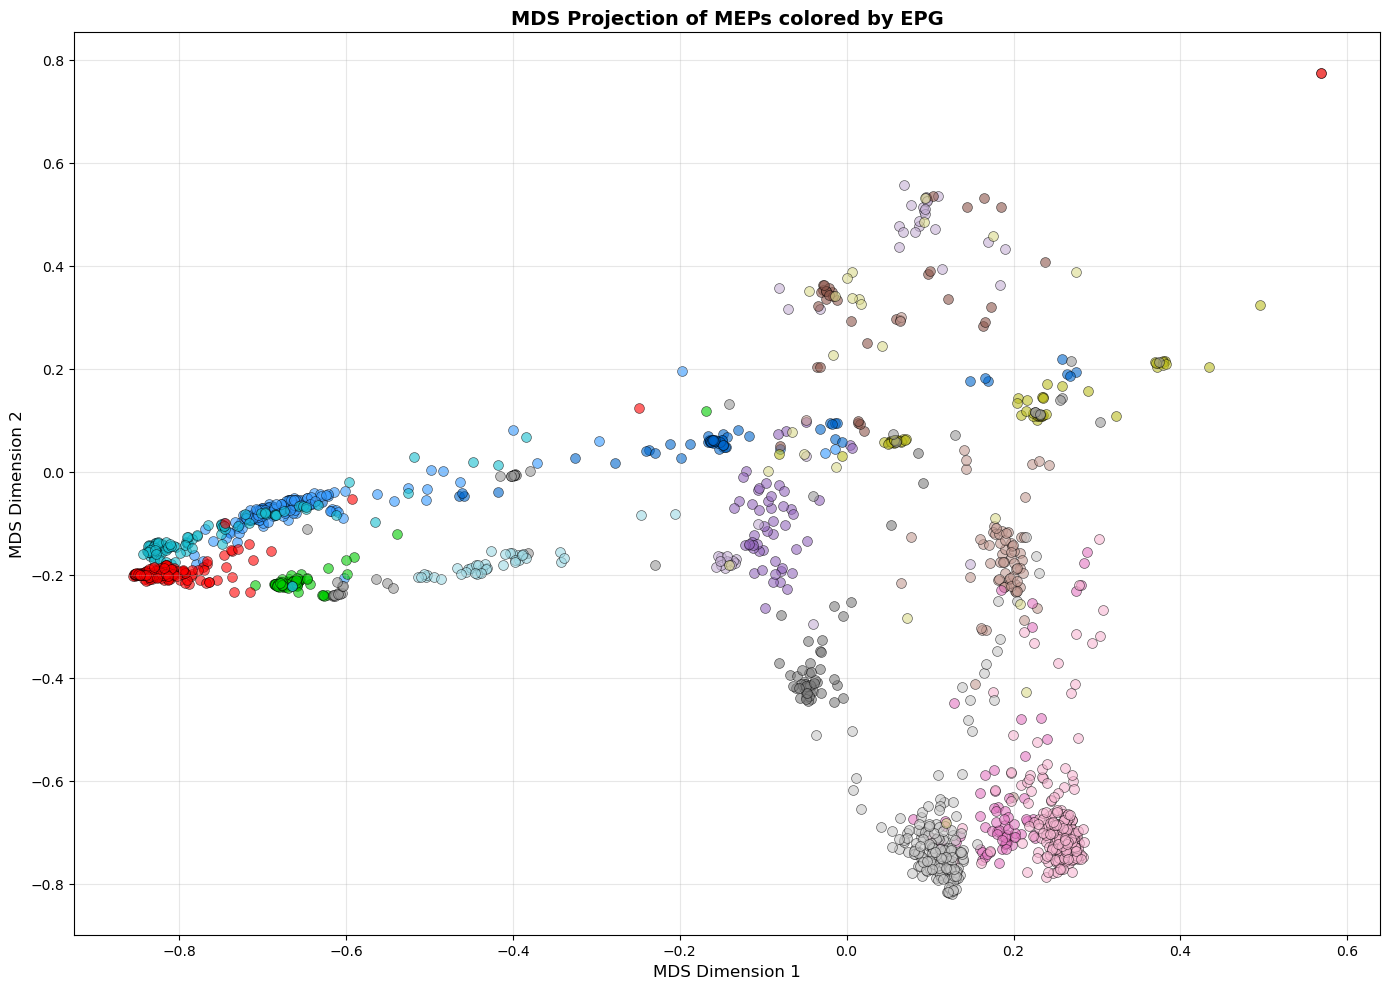
\includegraphics[width=0.8\linewidth]{imgs/D2-MEPS_by_EPG.png}
    \caption{MEPs colored by Political Group (EPG)}
\end{figure}
\begin{figure}[h!]
    \centering
    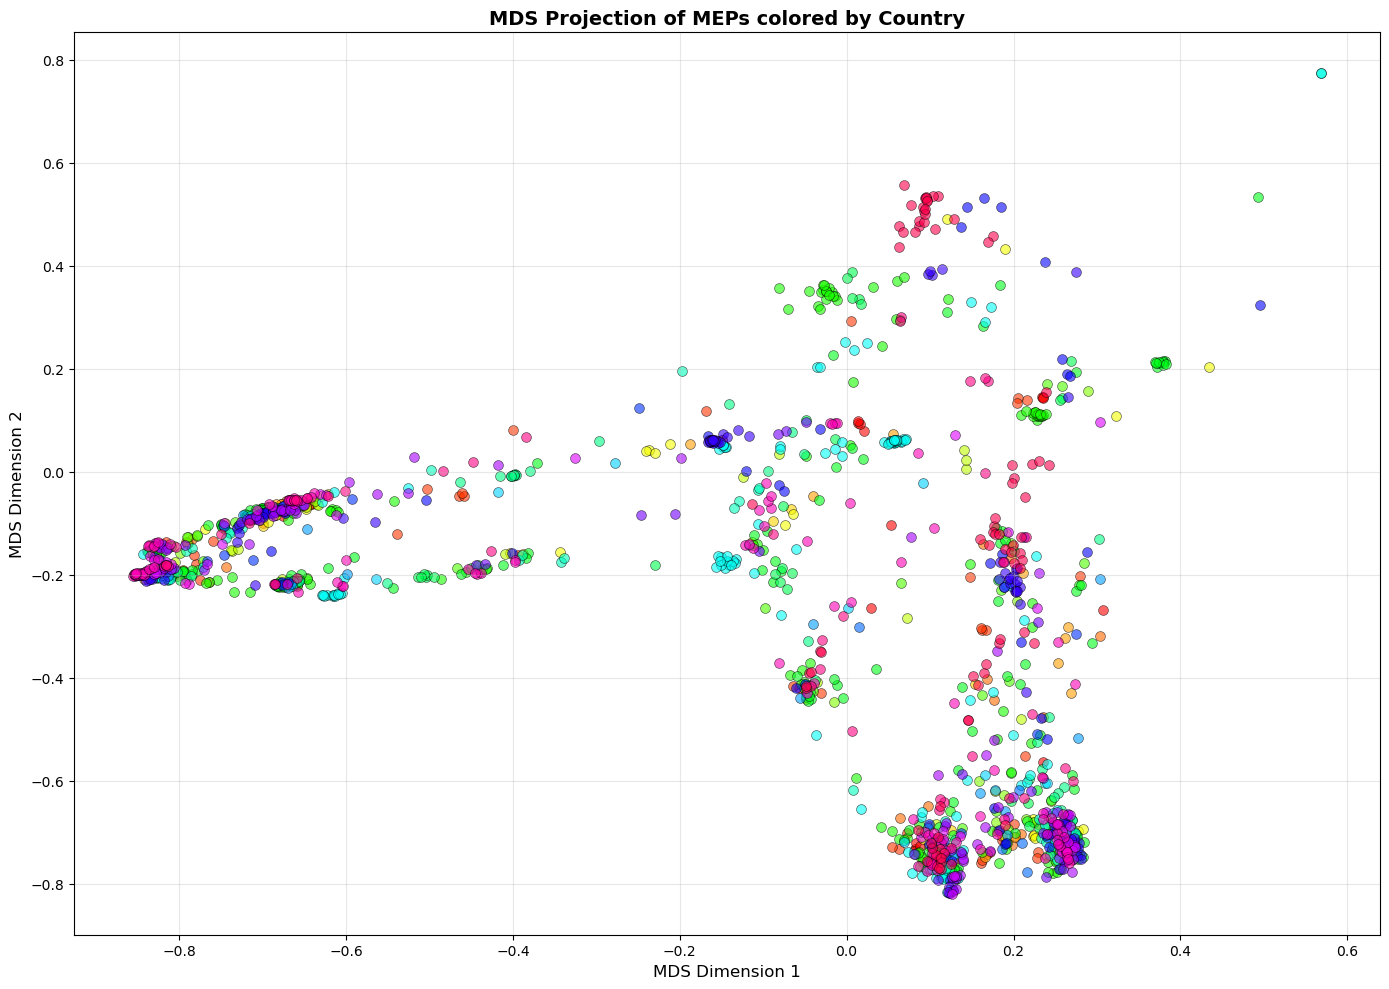
\includegraphics[width=0.8\linewidth]{imgs/D2-MEPS_by_Country.png}
    \caption{MEPs colored by Country}
\end{figure}
The MDS visualization reveals that political group (EPG) affiliation is the dominant factor explaining MEP voting patterns. When colored by EPG, the plot shows clear, well-separated clusters following a classic left-right political spectrum with a distinctive horseshoe pattern. In contrast, when colored by country, the visualization shows extensive overlap with no coherent national clusters.\\
This finding indicates that MEPs vote primarily along ideological lines rather than national interests. The strong cohesion within European political groups (e.g., EPP, S\&D) suggests that party discipline and shared political values transcend national boundaries in the European Parliament.\\
The horseshoe pattern is particularly noteworthy: the left-center-right spectrum is clearly visible, with centrist parties (EPP, Renew) at the top of the arc, left-wing parties (S\&D, Greens, GUE/NGL) on the left side, and right-wing/Eurosceptic parties (ECR, ID) on the right. The fact that political extremes appear closer to each other than to the center likely reflects their shared Eurosceptic positions despite opposite economic ideologies.

\subsection*{Question D.3}
In this section, we aim to conduct a more nuanced analysis of the MEP voting dataset by addressing the following research questions:

\begin{quote}
\emph{Do Members of the European Parliament (MEPs) tend to vote along party lines when a vote is sponsored by their own political group? Furthermore, which political groups exhibit systematic voting alliances?}
\end{quote}
Hypothesis:
\begin{itemize}
    \item Party loyalty $\rightarrow$  MEPs will vote overwhelmingly in favor of proposals sponsored by their own political group (high in-group support)
    \item Coalition patterns $\rightarrow$ certain political groups will consistently support each other's proposals, revealing stable legislative alliances (e.g., EPP-S\&D "grand coalition", or Greens-S\&D left-wing cooperation)
    \item Opposition patterns $\rightarrow$ ideologically distant groups will systematically vote against each other's proposals (e.g., far-left vs far-right, or Eurosceptics vs federalists)
\end{itemize}
\newpage
I used the support matrix with the dataset composed by EP9\_RCVs\_2022\_06\_22 and EP9\_Voted\_docs.
\\
Support matrix is a quantitative tool that measures how political groups vote on each other's legislative proposals. It is constructed as follows:
\begin{itemize}
    \item Rows $\rightarrow$ Political groups acting as sponsors (proposing votes/amendments)
    \item Columns $\rightarrow$ Political groups acting as voters (voting on those proposals)
    \item Cell values $\rightarrow$ support rate computed as $SupportRate = \frac{\text{Number of "For" votes by voter group}}{\text{Total votes cast by voter group}}$
\end{itemize}
\begin{figure}[h]
    \centering
    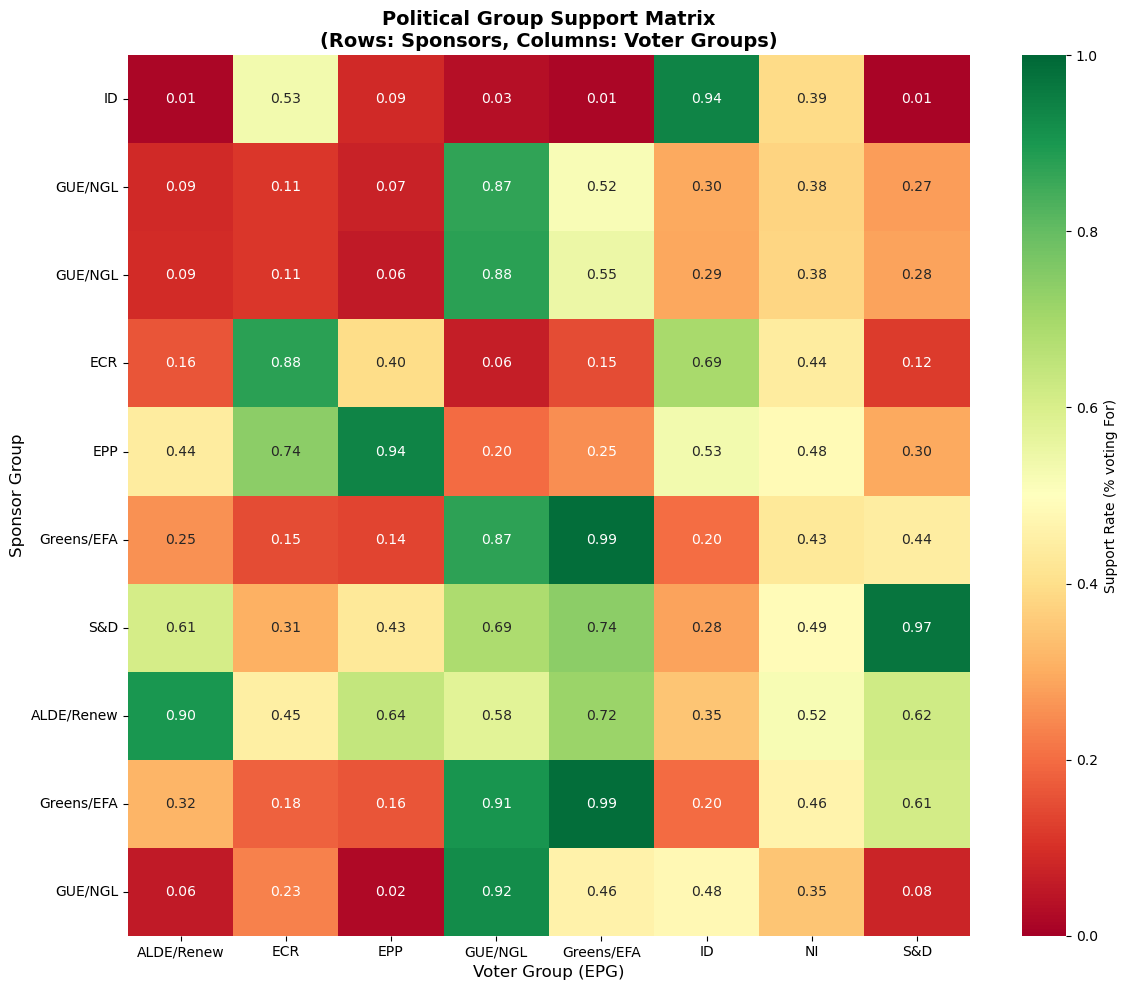
\includegraphics[width=0.7\linewidth]{imgs/D3-supportMatrix.png}
    \caption{Support Matrix}
\end{figure}
Metodology:
\begin{itemize}
    \item Step 1 $\rightarrow$ Data Integration
    \item Step 2 $\rightarrow$ Group Name Standardization: For each political group acting as sponsor: political groups have multiple naming variations across files (e.g., "EUL/NGL", "The Left", and "Confederal Group of the European United Left - Nordic Green Left" all refer to GUE/NGL). We created a mapping dictionary to standardize all group names to short, consistent labels.
    \item Step 3 $\rightarrow$ Vote Matching, for each political group acting as sponsor:
    \begin{itemize}
        \item Identified all votes in the Voted\_docs file where that group is listed as Author
        \item Matched these votes to the corresponding columns in the RCV file using position-based indexing
        \item Extracted the voting behavior of all MEPs on those specific votes
    \end{itemize}
    \item Step 4 $\rightarrow$ Support Rate Calculation, for each (sponsor, voter) pair
    \begin{itemize}
        \item Filtered votes to only those sponsored by the sponsor group
        \item Extracted how MEPs from the voter group voted on those proposals
        \item Applied the formula $\text{Support Rate} = \frac{(\text{\# of For votes})}{(\text{\# of For + Against + Abstain})}$
    \end{itemize}
\end{itemize}
Key findings:
\begin{itemize}
    \item \textbf{Very high in-group loyalty} across all groups (87-99\%), with Greens/EFA (99\%) and S\&D (97\%) showing the strongest discipline. This indicates that European political groups function as cohesive voting blocs with strong party discipline.
    \item \textbf{Three distinct voting blocks}
    \begin{itemize}
        \item Left alliance (S\&D , Greens/EFA , GUE/NGL): Mutual support ranging from 61-99\%
        \item Center-right coallition  (EPP , ECR): Moderate cooperation (40-74\%)
        \item Liberal bridge (ALDE/Renew): Supports both left and right groups moderately (62-72\%), acting as a swing voter
    \end{itemize}
    \item \textbf{Political isolatio of the far-right} The ID group (Identity and Democracy) receives near-zero support from all other groups (1-9\%), while maintaining high internal loyalty (94\%)
    \item \textbf{Grand Coalition} EPP and S\&D, traditionally the two largest groups, show asymmetric support (EPP→S\&D: 30\%, S\&D→EPP: 43\%). While they cooperate on major legislation, the moderate support levels confirm that ideological differences remain significant and coalition formation requires negotiation rather than automatic agreement. 
    \item \textbf{Strong left-wing cooperation} The highest cross-group support rates appear among left-wing groups, particularly Greens/EFA supporting GUE/NGL proposals (91-99\%), indicating that the left bloc votes together more cohesively than the right.
\end{itemize}
MDS showed that groups vote similarly while Support matrix shows who leads and who follows (e.g., Greens support S\&D proposals 74\%, but S\&D supports Greens 61\% - slightly asymmetric). This makes the support matrix analysis particularly valuable for understanding legislative effectiveness and coalition formation in the European Parliament rather than just having an overall ideological structure with MDS.

\end{document}